\begin{center}
\fbox{\fbox{\parbox{6.5in}{\centering
\begin{flushleft}

\vspace{2mm}
\hspace{5mm}
\textbf{\underline{Hulknurga mõiste}}

\vspace{2mm}
\hspace{5mm}
Hulknurk on tasandiline (2D) kujund, mis on piiratud kinnise murdjoonega.

\hspace{5mm}
Hulknurki liigitatakse nurkade (või külgede) järgi. Ehk: kolmnurk, nelinurk, viisnurk jne.


\vspace{2mm}
\hspace{15mm}
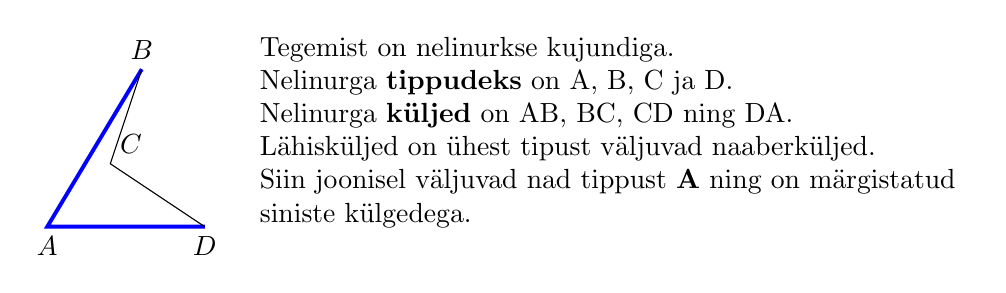
\begin{tikzpicture}[scale=0.4]
\draw[line width=0.50mm ,blue] (3,5) to (0,0)  to (5,0) ;
\draw (5,0) to (2,2) node[above right] {$C$}  to (3,5);
\node[above] at (3,5) {$B$};
\node[below] at (0,0) {$A$};
\node[below] at (5,0) {$D$};
\node[text width= 9cm] at (18,3)
{Tegemist on nelinurkse kujundiga.

Nelinurga \textbf{tippudeks} on A, B, C ja D.

Nelinurga \textbf{küljed} on AB, BC, CD ning DA.

Lähisküljed on ühest tipust väljuvad naaberküljed.

Siin joonisel väljuvad nad tippust \textbf{A} ning on märgistatud siniste külgedega.};
\end{tikzpicture}

\vspace{2mm}
\hspace{5mm}
Iga hulknurga \textbf{ümbermõõdu $P$} leidmiseks tuleb liita kõik hulknurga külgede pikkused kokku. Ehk

\vspace{2mm}
\hspace{5mm}
\begin{equation}
\fbox{$P = a+b+...+x$}
\end{equation}

\hspace{5mm}
kus tähed $a$, $b$, $c$ jne tähistavad hulknurga külgi.

\vspace{2mm}
\hspace{5mm}
Hulknurk võib olla ka \textbf{korrapärane}. See tähendab, et kõik tema küljed ja külgede vahelised nurgad on\\ \hspace{5mm} võrdsed. 

\vspace{5mm}
\hspace{5mm}
\textbf{\underline{Hulknurga sisenurkade summa}}

\vspace{2mm}
\hspace{5mm}
Üldine valem: \fbox{$s=(n-2)\cdot 180^{\circ} $}

\vspace{2mm}
\hspace{5mm}
kus $n$ - hulgnurga nurkade arv, $s$ - sisenurkade \textbf{summa}.

\vspace{2mm}
\hspace{5mm}
\textbf{Näiteks:} Leia \textbf{korrapärase} kaheksanurga üks sisenurk $\alpha$.

\vspace{2mm}
\hspace{5mm}
Teame, et tegemist on kaheksanurgaga, mis tähendab, et nurkade arv on $n=8$ ning et tegemist on\\ \hspace{5mm} korrapärase hulknurgaga. Korrapärane tähendas meil aga seda, et KÕIK selle kujundi nurgad on\\ \hspace{5mm} võrdsed. Järelikult, kui me leiame sisenurkade summa ja jagame selle nurkade arvuga läbi, siis leiame\\ \hspace{5mm} ühe nurga $\alpha$ väärtuse.

\vspace{2mm}
\hspace{5mm}
Leiame kaheksanurga sisenurkade summa:

\begin{equation}
\label{eq17_1}
s=(8-2)\cdot 180^{\circ} = 1080 ^{\circ}
\end{equation}

\hspace{5mm}
Kuna see on korrapärase kaheksanurga nurkade summa, siis ühe nurga leiame jagades summa 8 - ga:

\begin{equation}
\label{eq17_2}
\alpha = \dfrac{s}{8} = \dfrac{1080}{8} = 135^{\circ}
\end{equation}

\hspace{5mm}
Vastus: ühe nurga väärtus on $ \alpha = 135^{\circ} $

\end{flushleft}
}}}
\end{center}








\begin{center}
\fbox{\fbox{\parbox{6.5in}{\centering
\begin{flushleft}


\vspace{2mm}
\hspace{5mm}
\textbf{\underline{Rööpkülik ja selle omadused}}

\vspace{2mm}
\hspace{5mm}
Rööpkülik on nelinurk, mille...

\vspace{2mm}
\hspace{15mm}
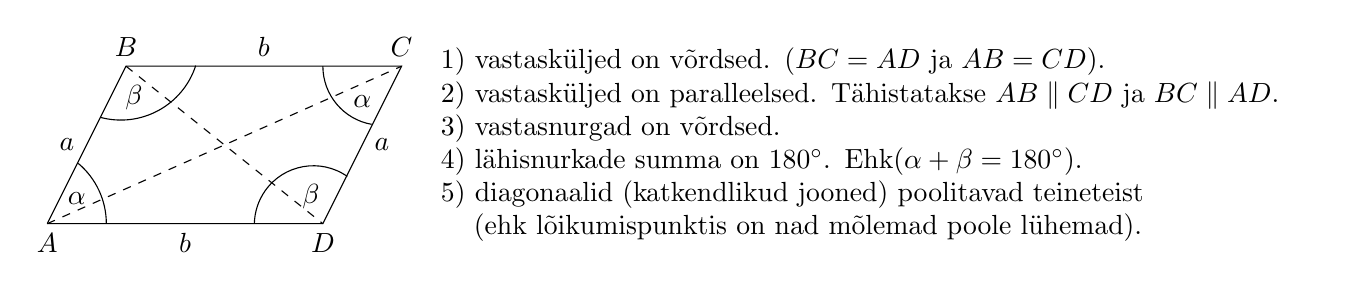
\begin{tikzpicture}[scale=0.5]
\draw (0,0) to (2,4) to (9,4) to (7,0) to (0,0);
\node at (0.5,2){$a$};
\node at (5.5, 4.5) {$b$};
\node at (8.5,2) {$a$};
\node at (3.5,-0.5) {$b$};
\node[below] at (0,0) {$A$};
\node[above] at (2,4) {$B$};
\node[above] at (9,4) {$C$};
\node[below] at (7,0) {$D$};
\draw (1.5,0) arc (0:50:2);
\node at (0.75,0.65) {$\alpha$};
\draw (7.62,1.2) arc (55:179:1.5);
\node at (6.7,0.7) {$\beta$};
\draw (1.35,2.7) arc (255:342:2);
\node at (2.2,3.2) {$\beta$};
\draw (7,4) arc (180:260:1.5);
\node at (8,3.1){$\alpha$};
\draw [dashed] (0,0) to (9,4);
\draw [dashed] (2,4) to (7,0);

\node[text width=11cm] at (21,2)
{1) vastasküljed on võrdsed. ($BC=AD$ ja $AB=CD$).

2) vastasküljed on paralleelsed. Tähistatakse $AB \parallel CD$ ja $BC \parallel AD$.

3) vastasnurgad on võrdsed.

4) lähisnurkade summa  on $180^{\circ}$. Ehk($\alpha + \beta = 180^{\circ}$).

5) diagonaalid (katkendlikud jooned) poolitavad teineteist\\ \hspace{3mm} (ehk lõikumispunktis on nad mõlemad poole lühemad).};
\end{tikzpicture}

\vspace{2mm}
\hspace{5mm}
\textbf{\underline{Rööpküliku pindala}}


\vspace{2mm}
\hspace{5mm}
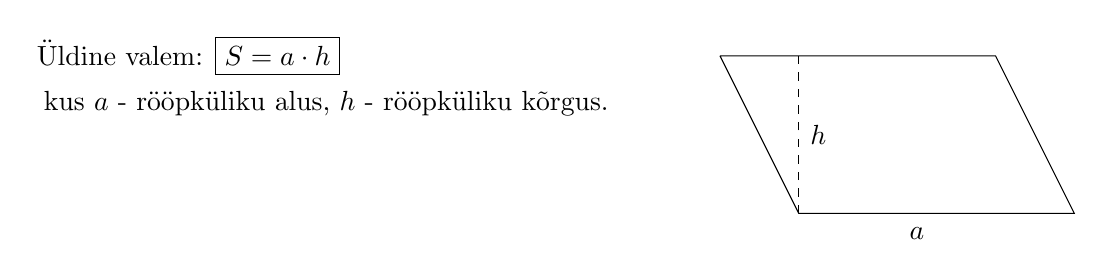
\begin{tikzpicture}[scale=0.5]
\draw (10,0) to (12,-4) to (19, -4) to (17,0) to (10,0);
\draw[dashed] (12, -4) to (12, 0);
\node at (15, -4.5) {$a$};
\node at (12.5, -2) {$h$};
\node at (-3.5,0) {Üldine valem: \fbox{$S=a\cdot h$}};
\node at (0,-1.2) {kus $a$ - rööpküliku alus, $h$ - rööpküliku kõrgus.};
\end{tikzpicture}

\hspace{5mm}
\textbf{\underline{Romb ja selle pindala}}

\vspace{2mm}
\hspace{5mm}
Kaks üldist valemit pindala arvutamiseks:

\vspace{2mm}
\hspace{5mm}
\begin{tikzpicture}[scale=0.5]

\node at (0,0) {\fbox{$S=a \cdot h$} \hspace{2mm} ja \hspace{2mm} \fbox{$S=\dfrac{d_{1} \cdot d_{2}}{2}$}};

\draw (10,-0.8) to (11,1) to (15,1) to (13,-2.6) to (9,-2.6) to (10,-0.8);
\draw[dashed,line width=0.40mm , red] (11,1) to (13, -2.6);
\draw[dashed, line width=0.40mm , blue] (15,1) to (9,-2.6);
\node[blue] at (11,-2) {$d_{1}$};
\node[red] at (12,0.3) {$d_{2}$};
\draw[dashed] (13,-2.6) to (13,1);
\node at (13.5, -0.8) {$h$};
\node at (12,1.3) {$a$};
\node at (14.5,-0.8) {$a$};
\node at (11,-3) {$a$};
\node at (9.5,-0.8) {$a$};
\end{tikzpicture}

\hspace{5mm}
Rombi puhul kehtivad kõik samad omadused, mis rööpküliku puhulgi, kuid mõned erinevused siiski on:

\vspace{2mm}
\hspace{5mm}
1) Rombi kõik küljed on võrdsed.

\hspace{5mm}
2) Rombi diagonaalid on risti (moodustavad $90^{\circ}$ nurga) ja poolitavad teineteist.

\hspace{5mm}
3) Romb on oma diagonaali suhtes sümmeetriline, mis ka tähendab, et rombi diagonaal poolitab rombi\\ \hspace{9.5mm} nurki.
\end{flushleft}
}}}
\end{center}


\vspace{0.5cm}

\textbf{Märkmed}\\
\vspace{2mm}
\begin{mdframed}[style=graphpaper]
\vspace{5cm}
\end{mdframed}

